\documentclass[11pt]{article}
\usepackage{listings}
\usepackage{amsfonts}
\usepackage{graphicx}
\newcommand{\numpy}{{\tt numpy}}    % tt font for numpy

\topmargin -.5in
\textheight 9in
\oddsidemargin -.25in
\evensidemargin -.25in
\textwidth 7in

\begin{document}

% ========== Edit your name here
\author{Francesco Penasa}
\title{Homework-5}
\maketitle

\medskip

% ========== Begin answering questions here
\begin{enumerate}

\item
\textbf{Exploit Integer Overflow vulnerability.}

% ========== Just examples, please delete before submitting
In order to exploit this vulnerability to get Iphone 11 Pro Max Max for free we have to insert a value in the variable \textit{item\_quantity} that makes the following equation true.
\begin{equation}
(x1500 + 1200) - y (2^{32}) = 0
\end{equation}
Where $x = $ \textit{item\_quantity} and $y \in \mathbb{N} > 0$.
The main obstacle to resolve this equation is to find x and y as positive integers, for this purpose we developed a simple Python3 script showed below.
\begin{lstlisting}[language=Python]
y = 0
overflow = (2**32) # integer max value + 1 in 32 bits.
while (True):
    y = y+1
    x = (y*overflow - 1200) / 1500
    if x == int(x):
        print("Found: " + str(x))
        break
\end{lstlisting}



This script tries all possible natural number greater than zero for the value $y$ and check if the resultant $x$ is an integer or a float/double number, if it is an integer print the $x$ and stop the cycle.\\
The result is: \textbf{214748364.0}\\
Inserting such result during the execution of the C code as input for the question \textit{"Great device, how many?"} will give us the following response: 
\textit{You solved the problem 
The Iphone Max Max is yours}.




\item
\textbf{Fix Integer Overflow vulnerability.} \\
To fix this vulnerabilities we check if \textit{item\_quantity} is greater than $10^{6}$.
\begin{lstlisting}[language=C]
if (item_quantity >= 1000000){
        printf("Overflow Risk!\n");
        return -1;
    }
\end{lstlisting}
This operation will grant us that the \textit{item\_quantity} variable will not reach the value 
\textbf{1431655} making it impossible for the \textit{price} variable (item\_quantity $* 1500 + 1200$) to exceed the \textbf{$2^{32}-1$} value and go in overflow.\\
In the following page the screenshot of its implementation in the C code is showed.


\begin{figure}
\centering
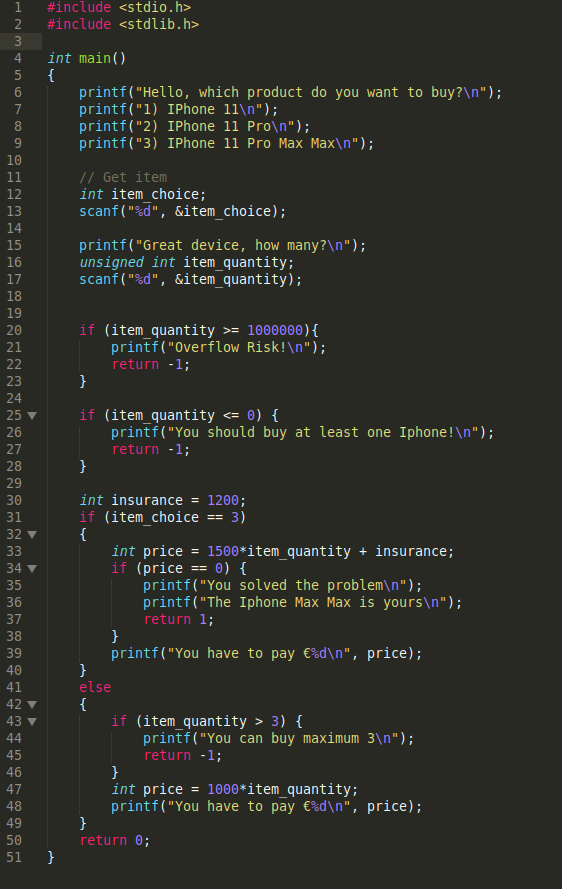
\includegraphics[scale=0.65]{image.png}
\end{figure}

\end{enumerate}
\end{document}
\grid
\grid